% \documentclass[OPTIONS]{CLASS}: Defines the overall layout of the document. Common classes are article, report, book.
\documentclass{article}

% \usepackage[OPTIONS]{PACKAGE}: Includes additional packages to extend LaTeX functionalities. Graphicx for example inserts functionalities for images. A good analogy for packages are libraries in other languages
\usepackage{graphicx} 

% \title{TITLE}: Defines the document title.
\title{LaTeX Cheat Sheet}
% \author{AUTHOR}: Defines the document author.
\author{Andrew Montalbano}
% \date{DATE}: Defines the document date.
\date{March 2024}

% Required for hyperlinks
\usepackage{hyperref}

% Required for color text
\usepackage{xcolor}

% Configure hyperlink colors
\hypersetup{
    colorlinks=true,
    urlcolor=blue,  % Color for URL links
    citecolor=black, % Color for citation links
    linkcolor=black, % Color for internal links
}

% Required for highlighting text
\usepackage{soul} 

% Required for bibliography management
\usepackage{biblatex}
% Add the bibliography file
\addbibresource{citations.bib} 

% Required for enhanced referencing
\usepackage{cleveref} 

% Required for subfigures
\usepackage{subcaption}

% Required for positioning floats
\usepackage{float} 

% Required for multiple columns
\usepackage{multicol} 

% Required for page layout
\usepackage[landscape]{geometry}

% Required for displaying keyboard shortcuts
\usepackage{menukeys} 

% \geometry{OPTIONS}: Sets page dimensions and margins. Example options are top, left, right, bottom.
\geometry{top=.5in,left=.5in,right=.5in,bottom=.5in}

% Turn off header and footer
\pagestyle{empty}

% Redefine section commands to use less space
% \renewcommand{\COMMAND}[ARGUMENTS]{NEW_DEFINITION}: Redefines an existing command with a new definition. We will use the following three commands to reduce the whitespace for the cheatsheet. Don't worry too much about these commands
\makeatletter
\renewcommand{\section}{\@startsection{section}{1}{0mm}%
                                {-1ex plus -.5ex minus -.2ex}%
                                {0.5ex plus .2ex}%x
                                {\normalfont\large\bfseries}}
\renewcommand{\subsection}{\@startsection{subsection}{2}{0mm}%
                                {-1explus -.5ex minus -.2ex}%
                                {0.5ex plus .2ex}%
                                {\normalfont\normalsize\bfseries}}
\renewcommand{\subsubsection}{\@startsection{subsubsection}{3}{0mm}%
                                {-1ex plus -.5ex minus -.2ex}%
                                {1ex plus .2ex}%
                                {\normalfont\small\bfseries}}
\makeatother

% Don't print section numbers
\setcounter{secnumdepth}{0}

% Set paragraph formatting
\setlength{\parindent}{0pt}
\setlength{\parskip}{0pt plus 0.5ex}

% \begin{ENVIRONMENT} ... \end{ENVIRONMENT}: Begins and ends an environment, such as document, section, figure.
\begin{document}

% Begin a four-column layout
\begin{multicols}{4} 

{\huge\LaTeX} is a powerful text editing suite. Here is a list of helpful commands!

% Uncomment the line below to add a table of contents
% \tableofcontents

% \section{TITLE}, \subsection{TITLE}, etc.: Creates a new section, subsection, etc., with the given title.
\section{Text Commands}

% To show LaTeX commands as text, we use the \verb command. This tells latex to directly print the text, and not to execute the commands. 
\subsection{Verbatim} 
\begin{center}
\begin{tabular}{ll}
\verb|\verb| & Print a single line of text exactly as typed \\
\verb|\begin{verbatim}| & Print multiple lines of text exactly as typed \\
\end{tabular}
\end{center}

% Commands for emphasizing text
\subsection{Text Emphasis}
\begin{center}
    \begin{tabular}{ll}
    % \textit command: Italicize text
\verb|\textit{text}| & \textit{Italicize text} \\
% \textbf command: Bold text
\verb|\textbf{text}| & \textbf{Bold text}\\
% \textsc command: Small caps text
\verb|\textsc{text}| & \textsc{Small Caps}\\
% \emph command: Emphasize text
\verb|\emph{text}| & \emph{Emphasized text}\\
% \underline command: Underline text
\verb|\underline{text}| & \underline{Underline text}
\end{tabular}
\end{center}

\vspace{-8pt}

% Commands for changing font size
\subsection{Font Size} 
\begin{center}
 \begin{tabular}{ll}
% \tiny command: Tiny text
\verb|\tiny|          &  \tiny{tiny text} \\
% \scriptsize command: Script size text
\verb|\scriptsize|    &  \scriptsize{scriptsize text} \\
% \footnotesize command: Footnote size text
\verb|\footnotesize|  &  \footnotesize{footnotesize text} \\
% \small command: Small text
\verb|\small|         &  \small{small text} \\
% \normalsize command: Normal size text
\verb|\normalsize|    &  \normalsize{normal size text} \\
% \large command: Large text
\verb|\large|         &  \large{large text} \\
% \Large command: Large text
\verb|\Large|         &  \Large{Large text} \\ 
% \LARGE command: LARGE text
\verb|\LARGE|         &  \LARGE{LARGE text} \\
% \huge command: Huge text
\verb|\huge|          &  \huge{huge text} \\
% \Huge command: Huge text
\verb|\Huge|          &  \Huge{Huge text}
\end{tabular}   
\end{center}

\vspace{-8pt}

% Commands for inline symbols
\subsection{Inline Symbols} 
\begin{tabular}{rl}
% \& command: Ampersand symbol
\verb|\&| & \& \\
% \textbar command: Vertical bar symbol
\verb|\textbar| & \textbar\\ 
% \textbackslash command: Backslash symbol
\verb|\textbackslash| & \textbackslash\\
% \% command: Percent symbol
\verb|\%| & \%\\
% \$ command: Dollar symbol
\verb|\$| & \$ 
\end{tabular}

% Commands for creating sections
\subsection{Sections}
Sections are made with \verb|\section|
\begin{center}
    \begin{tabular}{ll}
    % \section command: Create a new section
        \verb|\section{Title}| & {\large\textbf{Title}} \\
        % \subsection command: Create a new subsection
        \verb|\subsection{Title}| & {\normalsize\textbf{Title}} \\
        % \subsubsection command: Create a new subsubsection
        \verb|\subsubsection{Title}| & {\small\textbf{Title}} \\
    \end{tabular}
\end{center}

% Commands for controlling spacing
\subsection{Spacing} 
\begin{tabular}{ll}
% \vspace command: Move text vertically by specified amount
    \verb|\vspace{X}| & Move text vertically by X amount \\
    % \vfill command: Fill vertical space
    \verb|\vfill| & Fill vertical space\\
    % \\ command: Create a new line
    \verb|\\| & Create a new line\\
    % \newpage command: Create a new page
    \verb|\newpage| & Create a new page
\end{tabular}

% Commands for creating tables
\section{Tabular Commands} 
Create a table by:
\vspace{-5pt}
\begin{verbatim}
\begin{tabular}{cc}
    a & b  \\
    c & d
\end{tabular}
\end{verbatim}

% Commands for specifying column alignment
\subsection{Column Specifications} 
\begin{center}
\begin{tabular}{c|l|r}
    % c, l, and r specify center, left, and right alignment respectively
    center & left & right\\
    c & l & r\\
\end{tabular}   
\end{center}

% Adding horizontal lines with \hline and vertical lines with | in column alignment
Add horizontal lines with \verb|\hline| at the start or end of each row; or vertical lines with \verb!|! when setting column alignment

% Commands for creating equations
\section{Equations} 
Use \verb|$$| to place equations inline, or display them with \verb|\begin{equation}|

% Common math symbols
\subsection{Math Symbols} 
Symbols are produced with commands, usually their English name or an abbreviation of it
\begin{center}
\begin{tabular}{cc|cc}
    % \pi command: Pi symbol
    \verb|\pi| & $\pi$ & % \Pi command: Capital pi symbol
    \verb|\Pi| & $\Pi$ \\
    % \infty command: Infinity symbol
    \verb|\infty| & $\infty$ & % \pm command: Plus-minus symbol
    \verb|\pm| & $\pm$ \\
    % \hat command: Hat accent
    \verb|\hat a| & $\hat a$ & % \dot command: Dot accent
    \verb|\dot a| & $\dot a$
\end{tabular}    
\end{center}

% Common math operations


\subsection{Math Operations}
\begin{center}
\begin{tabular}{cc|cc}
    % \sum command: Summation symbol
    \verb|\sum| & $\sum$ & % \prod command: Product symbol
    \verb|\prod| & $\prod$ \\
    % \frac command: Fraction
    \verb|\frac{a}{b}| & $\frac{a}{b}$ & % \sqrt command: Square root
    \verb|\sqrt{a}| & $\sqrt{a}$
\end{tabular}
\end{center}

% Useful math environments
\subsection{Math Environments}
\begin{tabular}{ll}
% \begin{equation} command: Start an equation environment
    \verb|\begin{equation}| & Create an equation \\
% \begin{align} command: Start an align environment
    \verb|\begin{align}| & Create an aligned set of equations\\
% \begin{multline} command: Start a multline environment
    \verb|\begin{multline}| & Create a multi-line equation\\
\end{tabular}

% Required packages and their uses
\section{Useful Packages} 
Packages are included with \verb|\usepackage{packagename}| to include a package. 
\begin{tabular}{ll}
    % graphicx package: Required for including images
    \verb|graphicx| & Needed to include images \\
    % hyperref package: Required for hyperlinks
    \verb|hyperref| & Creates hyperlinks and references\\
    % xcolor package: Required for coloring text and links
    \verb|xcolor| & Colors hyperlinks\\
    % biblatex package: Required for citations and bibliography
    \verb|biblatex| & Citations and bibliography\\
    % cleveref package: Required for enhanced referencing
    \verb|cleveref| & Better references\\
    % subcaption package: Required for subfigures
    \verb|subcaption| & Needed for subfigures\\
    % float package: Required for positioning floats
    \verb|float| & Floats images
\end{tabular}

% Commands for managing citations
\section{Biblatex} 
The bibtex citation of an article looks like:
\begin{verbatim}
@article{Ref Name,
  title={Paper title},
  author={Authors},
  journal={A good Journal},
  year={Year},
}
\end{verbatim}
Place all of them in a new file called \verb|citations.bib|. Then:
\begin{tabular}{ll}
   % \cite command: Cite a paper
   \verb|\cite| & Cite a paper \\
   % \parencite command: Cite a paper with parentheses
   \verb|\parencite| & (Cite a paper)\\
   % \printbibliography command: Print the bibliography
   \verb|\printbibliography| & Display the bibliography
\end{tabular}

% Overleaf shortcuts
\section{Overleaf Short-cuts}
\begin{tabular}{ll}
    % ctrl + enter: Compile document
    \verb|ctrl + enter| & Compile document \\
    % ctrl + /: Comment section
    \verb|ctrl + /| & Comment section\\
    % ctrl + b: Bold text
    \verb|ctrl + b| & \textbf{Bold}\\
    % ctrl + i: Italicize text
    \verb|ctrl + i| & \textit{Italicize}\\
    % ctrl + U: Convert text to uppercase
    \verb|ctrl + U| & UPPERCASE\\
    % ctrl + shift + U: Convert text to lowercase
    \verb|ctrl + shift + U| & lowercase\\
    % ctrl + space: Autocomplete command
    \verb|ctrl + space| & Autocomplete\\
    % alt + shift + up-arrow or down-arrow: Move line up or down
    \verb|alt + shift + |\arrowkey{^} & Move line
\end{tabular}
* Use \cmd\ instead of \verb|ctrl| on Mac
\vfill

% Commands for creating figures
\section{Figures} 
To create a figure, use \verb|\begin{figure}|
\begin{figure}[H]
    \centering
    % \includegraphics command: Include an image
    
\includegraphics[width=0.3\linewidth]{Subject.png}
    % \caption command: Add a caption to the figure
    \caption{Tofu!}
    % \label command: Add a label to the figure for referencing
    \label{fig:enter-label}
\end{figure}

% \subfigure command: Create subfigures side-by-side, requires subcaption package
Use \verb|\subfigures| to make figures side-by-side, needs package \verb|subcaption|
\begin{figure}[H]
     \centering
     \begin{subfigure}{0.49\linewidth}
         \centering
         % \includegraphics command: Include an image
         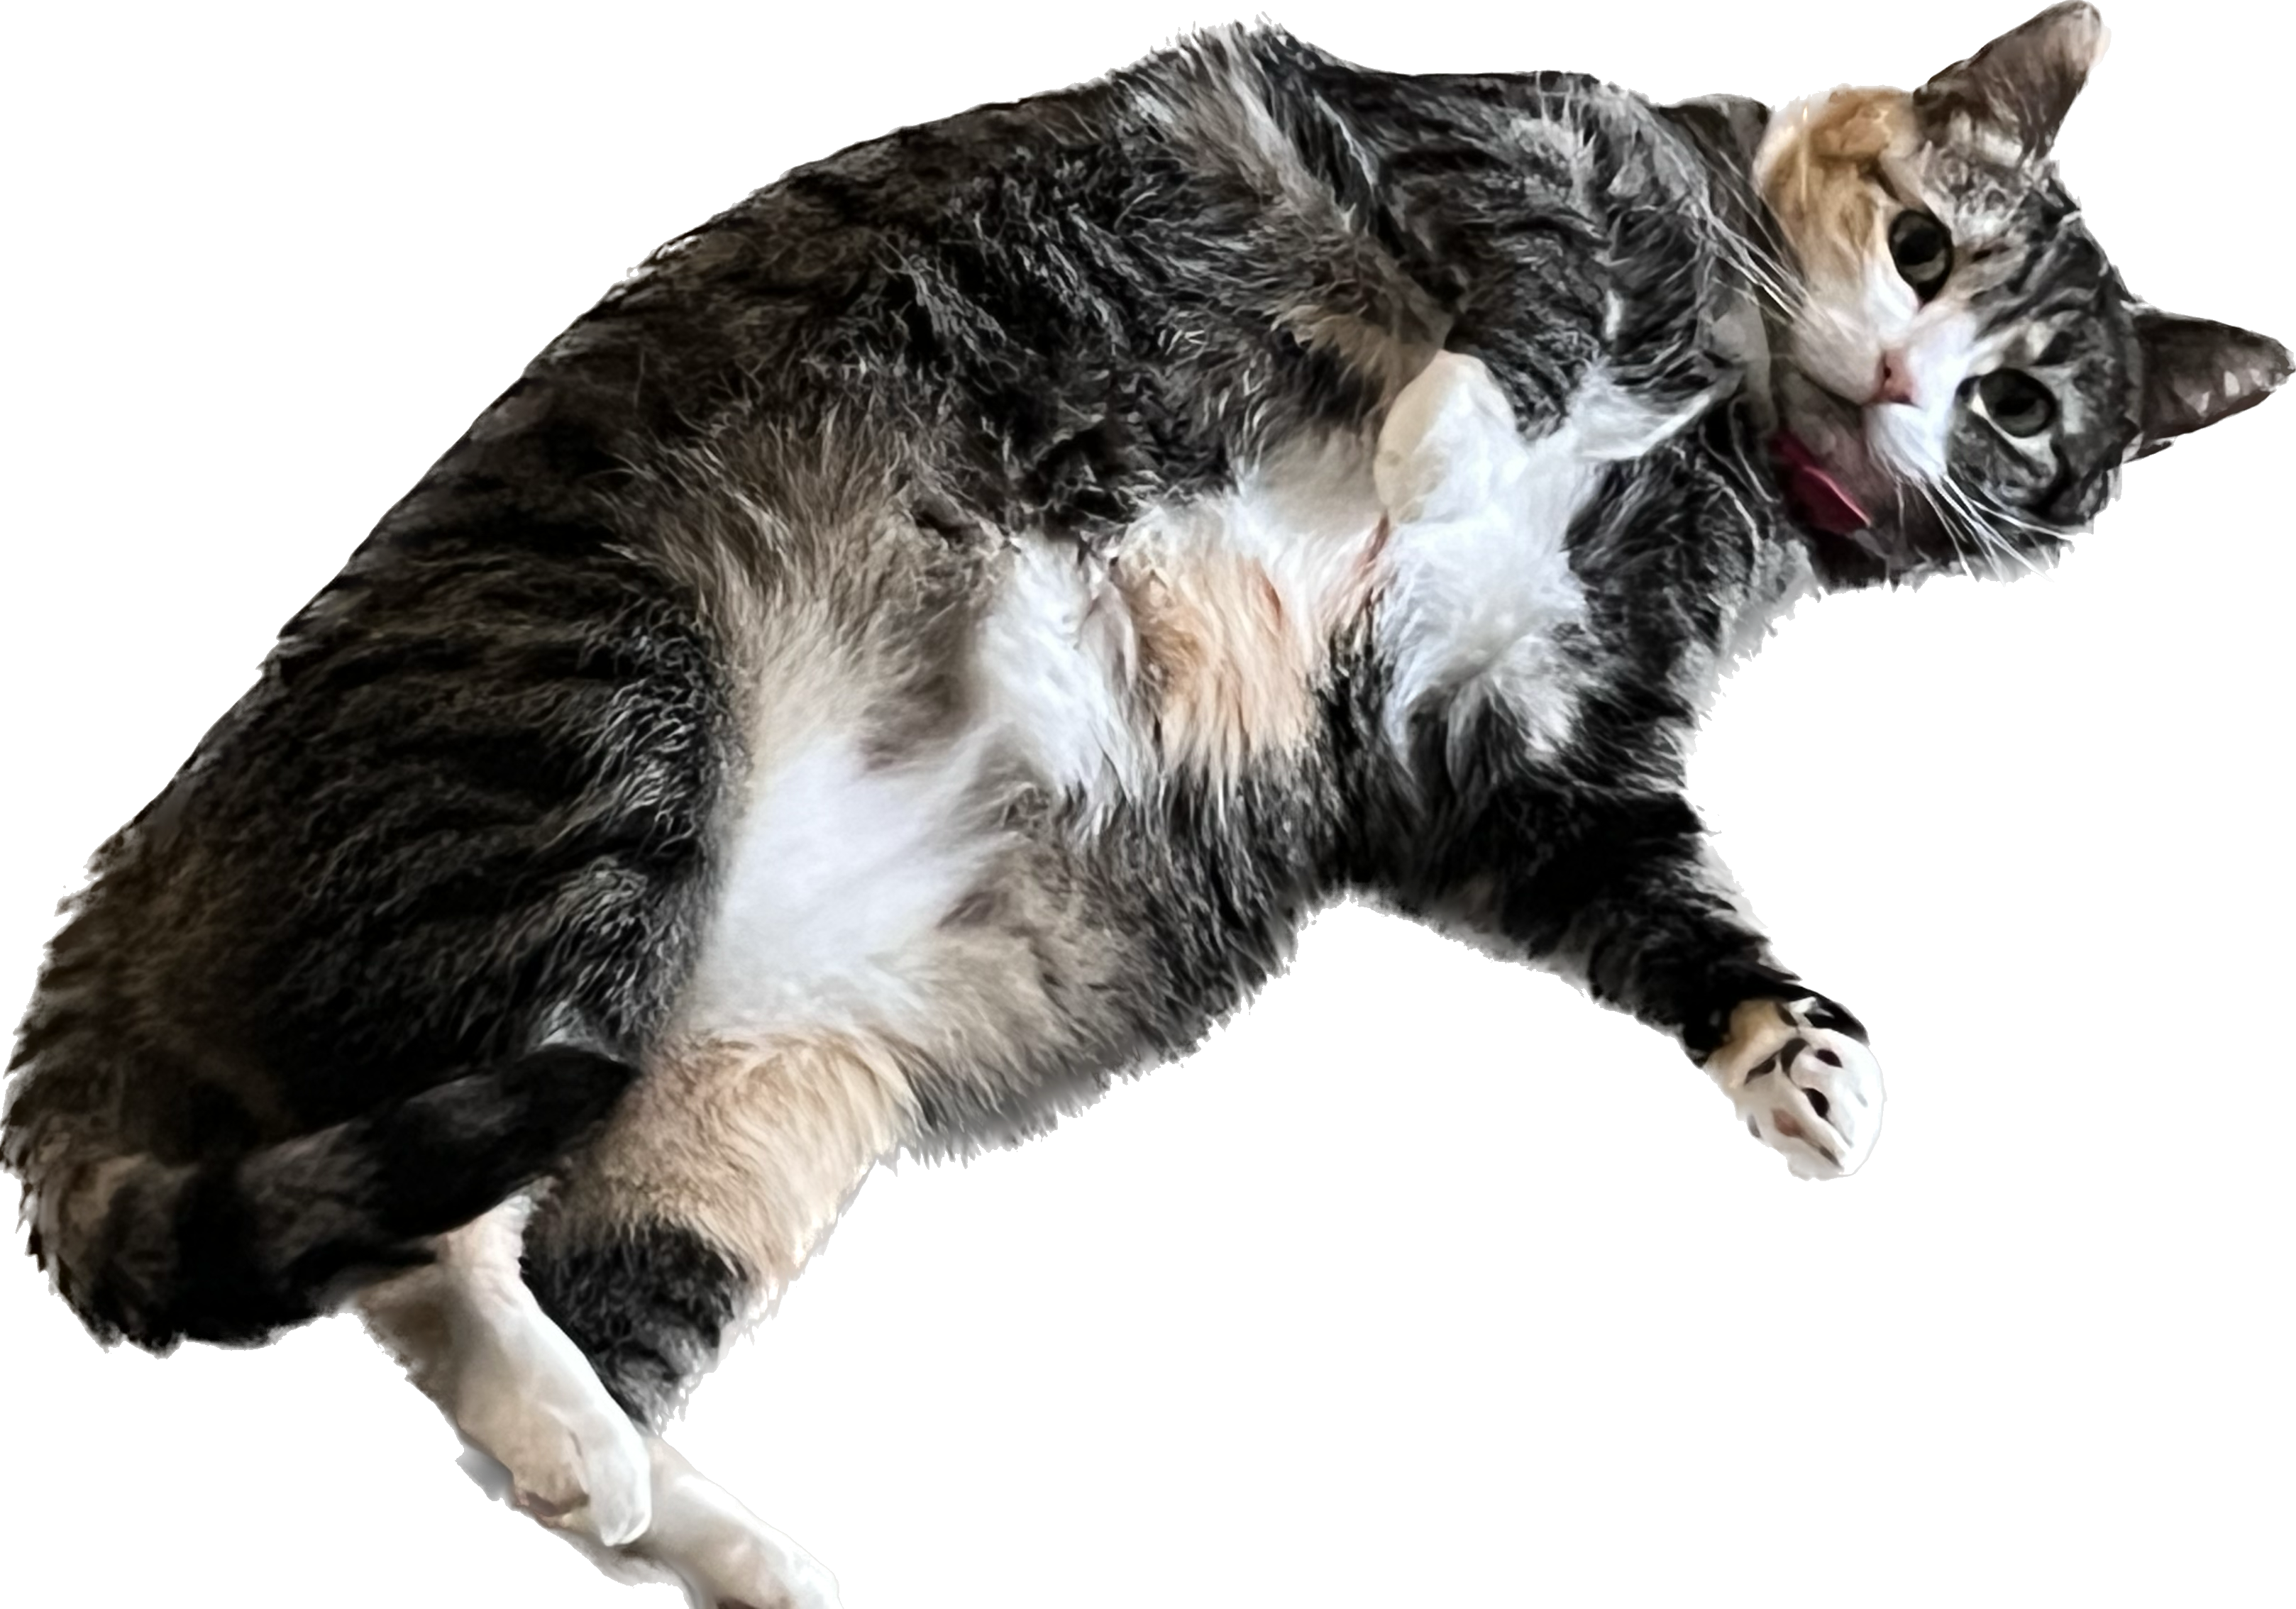
\includegraphics[width=\linewidth]{Subject 3.png}
         % \caption command: Add a caption to the subfigure
         \caption{Meow}
         % \label command: Add a label to the subfigure for referencing
         \label{imgA}
     \end{subfigure}
     \hfill
     \begin{subfigure}{0.49\linewidth}
         \centering
         % \includegraphics command: Include an image
         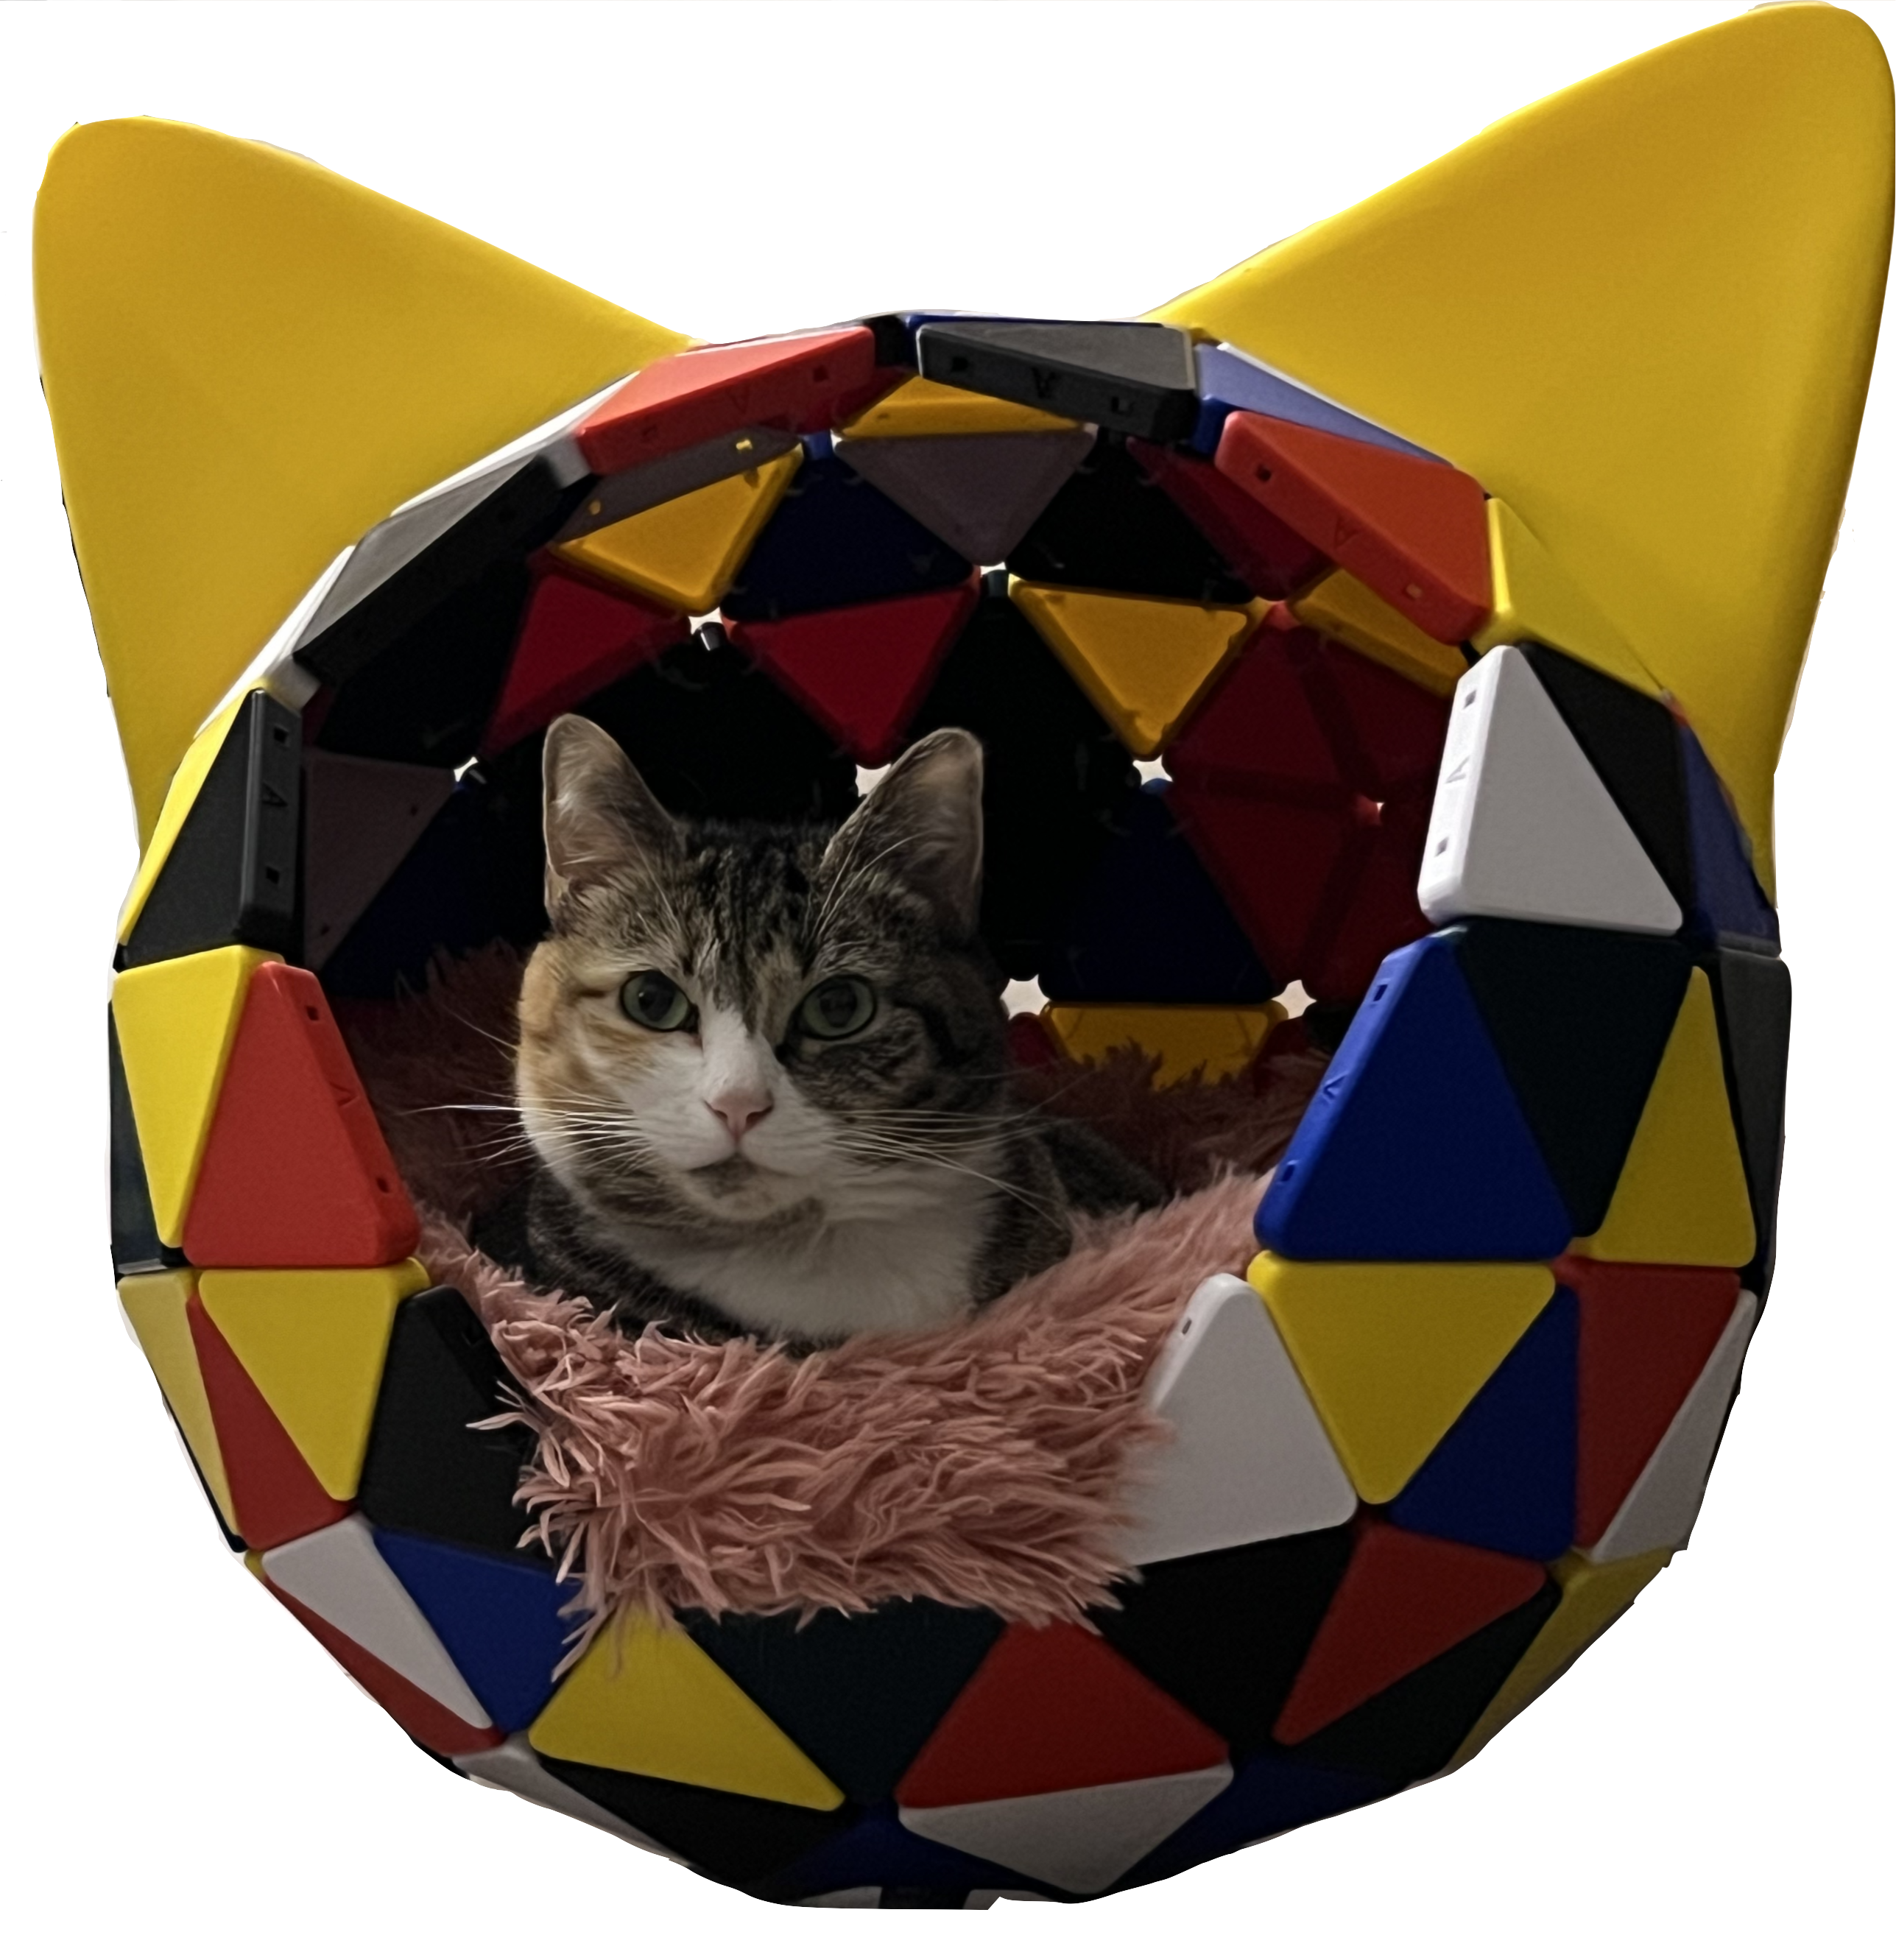
\includegraphics[width=\linewidth]{IMG_0546 2.png}
         % \caption command: Add a caption to the subfigure
         \caption{Tofu's House}
         % \label command: Add a label to the subfigure for referencing
         \label{imgB}
     \end{subfigure}
        % \caption command: Add a caption to the figure
        \caption{Tofu relaxing}
        % \label command: Add a label to the figure for referencing
        \label{fig:twoImages}
\end{figure}

% Commands for scaling images
To scale the image, we commonly scale its width to match the page width, but we can also scale the image overall.
\begin{tabular}{ll}
    % width option: Set the image width
    \verb|width=\textwidth| & Sets image width\\
    % scale option: Scale the image by a specified factor
    \verb|scale=NUM| & Scales by NUM 
\end{tabular}

% Commands for creating lists
\section{List Items} 
To create lists of things, we can use either \verb|enumerate| or \verb|itemize|
\vspace{-8pt}
\begin{enumerate}
    % \enumerate command: Create a numbered list
    \item \verb|enumerate| creates a numbered list
    \itemsep0em 
    % \itemize command: Create a bulleted list
    \item \verb|itemize| creates a bulleted list
    \itemsep0em 
    \begin{itemize}
        \item They can be nested!
    \end{itemize}
\end{enumerate}

% Commands for creating and modifying macros
\section{Commands} 
For repeated operations, a macro can be created with \verb|\newcommand{}[]{}|. 
Example: \verb|\newcommand{\hello}{Hello!}|

These or existing commands can be modified by \verb|\renewcommand{}{}|. Example: 
\verb|\renewcommand{\hello}{Bonjour!}|

\end{multicols}

\end{document}
